
\chapter{REFERENCIAL TEÓRICO}


\section{Exemplo de figura}
 
    A Figura \ref{estruturaBPM}  mostra uma visão simplificada do funcionamento dos sistemas BPM.
    \begin{figure}[H]
        \centering
        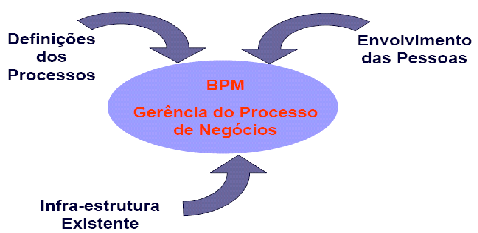
\includegraphics[scale=0.6,angle=0]{img/EstruturaBPM.png}
        \caption{Visão geral de um BPMS}
        \label{estruturaBPM}
    \end{figure}

\section{Exemplo de tabela}

	A Tabela \ref{tabFluxoUsa} mostra as atividades que compõem o fluxo de usabilidade e o papel requerido ao agente para realizá-las. As atividades de Análise de contexto de uso e Avaliação de usabilidade são decompostas em sub-fluxos, suas descrições são mostradas nas Tabelas \ref{tabAna} e \ref{tabAval}, respectivamente.

    \begin{table}[h]
        \begin{center}
    		\begin{tabular}{|c|c|}
    			\hline
                \textbf{Atividade} & \textbf{Papel requerido} \\ \hline
    			Planejamento & Gerente de Usabilidade \\
    			Controle  & \\
    			\hline
                Análise de contexto de uso &  \\
                Definição das funções do produto &  \\
                Prototipação de requisitos de interface & Analista de Usabilidade \\
                Definição de requisitos e metas de usabilidade & \\
                Revisão da análise de usabilidade & \\
                \hline
                Definição do estilo de interação & \\
                Desenho da interação & Arquiteto de usabilidade \\
                Revisão do desenho da interação & \\
                \hline
                Avaliação de usabilidade & Avaliador de Usabilidade  \\
                \hline
                Balanço final & Gerente de Usabilidade  \\
                \hline
    			%\multicolumn{3}{l}{\scriptsize Fonte: Indicar procedência.}\\
    			%\multicolumn{3}{l}{\scriptsize Notas: Alguma especificação geral.}\\
    			%\multicolumn{3}{l}{\scriptsize (1) Alguma nota específica}
    		\end{tabular}
    		\caption{Atividades do fluxo de usabilidade}
        	\label{tabFluxoUsa}
    	\end{center}
    \end{table}

    \begin{table}[h]
        \begin{center}
    		\begin{tabular}{|c|c|}
    			\hline
                \textbf{Atividade} & \textbf{Papel requerido} \\ \hline
    			Planejamento &  \\
                Preparação &  \\
                Modelagem preliminar de  usuários  &  \\
                Refinamento da modelagem de usuários &   \\
                Definição do modelo mental & Analista de Usabilidade  \\
                Análise de produtos concorrentes &  \\
                Modelagem preliminar de tarefas &  \\
                Refinamento da modelagem de tarefas &  \\
                Balanço final &  \\
                \hline
    			%\multicolumn{3}{l}{\scriptsize Fonte: Indicar procedência.}\\
    			%\multicolumn{3}{l}{\scriptsize Notas: Alguma especificação geral.}\\
    			%\multicolumn{3}{l}{\scriptsize (1) Alguma nota específica}
    		\end{tabular}
    		\caption{Atividades do sub-fluxo de análise de contexto de uso}
        	\label{tabAna}
    	\end{center}
    \end{table}

    \begin{table}[h]
        \begin{center}
    		\begin{tabular}{|c|c|}
    			\hline
                \textbf{Atividade} & \textbf{Papel requerido} \\ \hline
    			Planejamento &  \\
                Desenho &  \\
                Implementação &  \\
                Execução & Avaliador de Usabilidade  \\
                Análise dos dados &  \\
                Verificação do término &  \\
                Balanço final &  \\
                \hline
    			%\multicolumn{3}{l}{\scriptsize Fonte: Indicar procedência.}\\
    			%\multicolumn{3}{l}{\scriptsize Notas: Alguma especificação geral.}\\
    			%\multicolumn{3}{l}{\scriptsize (1) Alguma nota específica}
    		\end{tabular}
    		\caption{Atividades do sub-fluxo de avaliação de usabilidade}
        	\label{tabAval}
    	\end{center}
    \end{table}

